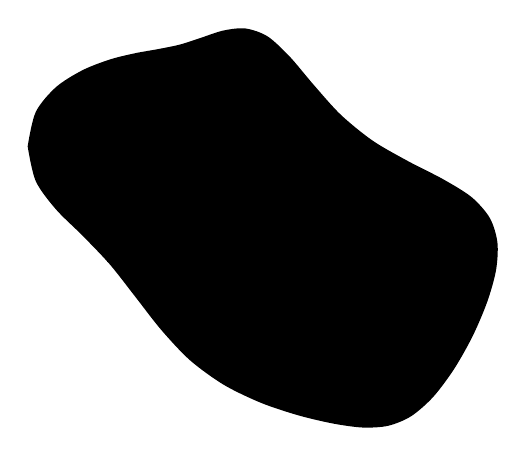
\begin{tikzpicture}[yscale=.6]%[width=\marginparwidth+25pt]
%\begin{axis}[width=\marginparwidth+25pt,%
%tick label style={font=\scriptsize},axis y line=middle,axis x line=middle,name=myplot,axis on top,%
%			%x=.37\marginparwidth,
%			%y=.37\marginparwidth,
%			xtick={1,2,3,4,5,6,7,8,9,10,11,12},% 
%%			extra x ticks={12.57},
%%			extra x tick labels={$4\pi$},
%%			ytick=\empty,
%			%minor y tick num=1,%extra y ticks={-5,-3,...,7},%
%%			minor x tick num=4,
%			ymin=-.1,ymax=8.5,%
%			xmin=-.1,xmax=12.5%
%]

\draw [{\colorone},thick,fill={\coloronefill},smooth] plot coordinates {(0,2.)(0.1013,2.717)(0.3567,3.238)(0.6934,3.594)(1.039,3.818)(1.355,3.948)(1.646,4.035)(1.925,4.132)(2.2,4.28)(2.475,4.428)(2.75,4.471)(3.025,4.307)(3.305,3.88)(3.607,3.287)(3.952,2.652)(4.361,2.098)(4.815,1.661)(5.253,1.285)(5.614,0.9071)(5.843,0.4705)(5.938,-0.04167)(5.919,-0.6295)(5.807,-1.293)(5.624,-2.009)(5.389,-2.703)(5.125,-3.29)(4.849,-3.692)(4.562,-3.892)(4.243,-3.929)(3.871,-3.846)(3.432,-3.674)(2.956,-3.409)(2.484,-3.028)(2.057,-2.511)(1.692,-1.869)(1.363,-1.168)(1.039,-0.4819)(0.6934,0.1248)(0.3567,0.679)(0.1013,1.273)(0,2.)};

\draw (1,3.8) -- (1,-.45) node [shift={(-3pt,0pt)},rotate=90,pos=.5] {\scriptsize 4.25};
%
\draw (2,4.15) -- (2,-2.45) node [shift={(-3pt,0pt)},rotate=90,pos=.5] {\scriptsize 6.6};

\draw (3,4.3) -- (3,-3.4) node [shift={(-3pt,0pt)},rotate=90,pos=.5] {\scriptsize 7.7};

\draw (4,2.6) -- (4,-3.85) node [shift={(-3pt,0pt)},rotate=90,pos=.5] {\scriptsize 6.45};

\draw (5,1.45) -- (5,-3.45) node [shift={(-3pt,0pt)},rotate=90,pos=.5] {\scriptsize 4.9};

%\end{axis}
%
%\node [right] at (myplot.right of origin) {\scriptsize $x$};
%\node [above] at (myplot.above origin) {\scriptsize $y$};
\end{tikzpicture}


